\documentclass[12pt,letterpaper]{exam}
\usepackage[lmargin=1in,rmargin=1in,tmargin=1in,bmargin=1in]{geometry}
\usepackage{../style/exams}

% -------------------
% Course & Exam Information
% -------------------
\newcommand{\course}{MAT 108: Exam 1}
\renewcommand{\term}{Fall -- 2023}
\newcommand{\examdate}{10/03/2023}
\newcommand{\timelimit}{85 Minutes}

\setbool{hideans}{true} % Student: True; Instructor: False

% -------------------
% Content
% -------------------
\begin{document}

\examtitle
\instructions{Write your name on the appropriate line on the exam cover sheet. This exam contains \numpages\ pages (including this cover page) and \numquestions\ questions. Check that you have every page of the exam. Answer the questions in the spaces provided on the question sheets. Be sure to answer every part of each question and show all your work. If you run out of room for an answer, continue on the back of the page --- being sure to indicate the problem number.} 
\scores
\bottomline
\newpage

% ---------
% Questions
% ---------
\begin{questions}

% Question 1
\newpage
\question[10] Suppose that the current CPI is 307.026. Further, suppose that the CPI next year at this time will be 319.307. 
	\begin{enumerate}[(a)]
	\item Find the inflation rate from this year to next year. 
	\item Estimate the cost of a good next year that currently costs \$29.99. 
	\item If this inflation rate continue across the next decade, what will be percentage increase in costs ten years from now compared to now?
	\end{enumerate}



% Question 2
\newpage
\question[15] Consider the revenue function, $R(q)$, and cost function, $C(q)$, for some good given in the plot below. 
	\[
	\fbox{
	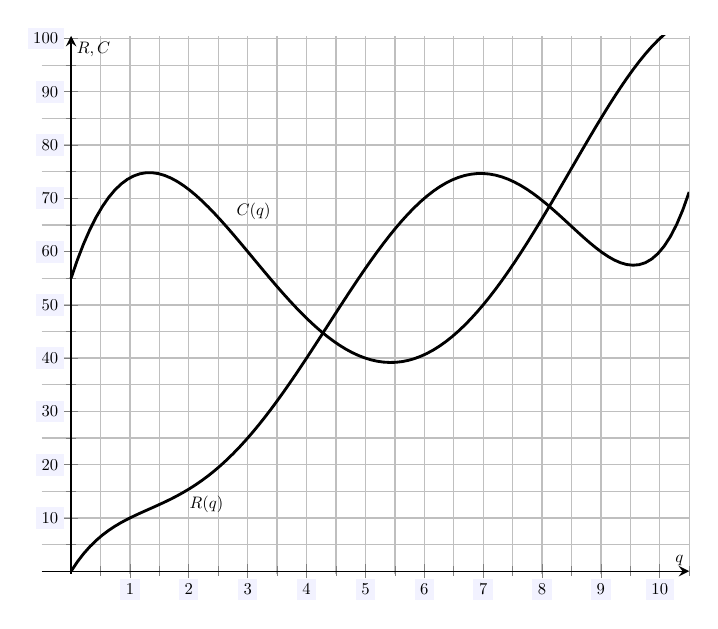
\begin{tikzpicture}[scale=1.2,every node/.style={scale=0.5}]
	\begin{axis}[
	grid=both,
	axis lines=middle,
	ticklabel style={fill=blue!5!white},
	xmin= -0.5, xmax=10.5,
	ymin= -0.5, ymax=100.5,
	xtick={0,1,2,...,11},
	ytick={0,10,20,...,100},
	minor x tick num = 1,
	minor y tick num = 1,
	xlabel=\(q\),ylabel=\({R,C}\),
	]
	\node at (2.3,12.5) {$R(q)$};
	\addplot[domain=0:10.5, samples=100,line width=0.03cm] 
	(x, 17.6667*x - 11.3056*x^2 + 4.16204*x^3 - 0.546296*x^4 + 0.0231481*x^5);
	\node at (3.1,67.5) {$C(q)$};
	\addplot[domain=0:10.5, samples=100,line width=0.03cm] 
	(x, 55 + 33.994*x - 17.7014*x^2 + 2.69544*x^3 - 0.131944*x^4 + 0.000992063*x^5);
	\end{axis}
	\end{tikzpicture}
	}
	\] 
In the plot above, the number of goods produced, $q$, is measured in tens of thousands of items and the outputs of $R(q)$ and $C(q)$ are measured in tens of thousands of dollars. Given this data, answer the following:
	\begin{enumerate}[(a)]
	\item What are the fixed costs?
	\item What the break-even point(s)?
	\item Is the company experiencing profit or loss for this good at a production level of 65,000~units?
	\item Estimate the profit or loss in (c). 
	\item  Estimate the average revenue per sale at a production/sale level of 70,000~units. 
	\end{enumerate}



% Question 3
\newpage
\question[15] Kriss Crosse is taking out a loan to expand her applesauce business. The bank offers her a \$260,000 loan at 14.6\% annual interest, compounded monthly. By accepting the loan terms, Ms. Crosse will pay \$30,000 up-front. The remainder of the loan will be repaid with equal, end of the month payments of \$4,074.38 over 8~years
	\begin{enumerate}[(a)]
	\item How much will Kriss still owe on the loan after 6~years of payments?
	\item How much interest will Kriss pay in total for this loan?
	\end{enumerate}



% Question 4
\newpage
\question[15] Braden Haire is investing some of the profits from his politically active wig company Wigs for Whigs. He places \$65,000 into an account that advertises a 4.15\% annual interest rate, compounded continuously. 
	\begin{enumerate}[(a)]
	\item One year from now, by what percentage would Braden's money have increased?
	\item Assuming Braden makes no additional deposits into the account, how much will be in the account after 33~years?
	\item How much interest would the account have earned after 33~years?
	\end{enumerate}



% Question 5
\newpage
\question[15] Emma Minat needs some quick cash by the end of next year to help fund her growing addiction to soap carving. She estimates that she will need at least \$8,500 to fund her newest series of soapy endeavors. Emma finds a new type of bond that offers 3.35\% annual interest, compounded weekly. 
	\begin{enumerate}[(a)]
	\item How much should she take out in these bonds to have the necessary \$8,500 by the end of the two years?
	\item How much longer would Emma have to let these bonds accrue interest before they are worth \$10,000?
	\end{enumerate}



% Question 6
\newpage
\question[15] Doug Graves needs to have repairs made to his hearse for his mortuary Look Alive. The reaches out to a bank for a loan to fund the repairs. The bank offers a \$2,500 discount note for 9~months at 9.4\% annual interest.
	\begin{enumerate}[(a)]
	\item How much would Mr. Graves receive from the bank, if he took the loan?
	\item At the end of the 9~months, how much would Mr. Graves owe the bank?
	\end{enumerate}



% Question 7
\newpage
\question[15] Neil Downe is starting a college fund for their son, Stan. Every 3~months, at the start of the month, they place \$960 into an account that earns 5.13\% annual interest, compounded monthly. How much will the account have after 18~years, assuming no other funds have ever been placed into the account beyond these deposits. 


\end{questions}
\end{document}